%!TEX root = ../index.tex
Von Beginn der Arbeit waren zwei Daten klar. Zum einen sollte die Arbeit vom 16.4.2012 bis am 4.5.2012 unterbrochen werden da ich in dieser Zeit meinen letzten ``Fortbildungsdienst der Truppe''\footnote{\url{http://www.vtg.admin.ch/internet/vtg/de/home/militaerdienst/dienstleistende/dienstleistungspflicht/sdt.html}} bei der Schweizer Armee leisten musste. Anderseits war auch von Anfang an klar, dass ich die Arbeit spätestens in der Woche vom 16.7.2012 abgeben werde, da ich danach drei Wochen abwesend sein werde.

\section{Projektplan}
\label{sec:projektplan}
Das Projekt wurde nur auf Wochen genau geplant, da zu Beginn der Arbeit nicht klar war, wann ich wie viel Zeit in die Arbeit investieren kann. Diese Planung ist in Abbildung~\ref{fig:zeitplan} zu sehen. Die gesetzten Meilensteine wurden nicht alle Termingerecht erreicht. Jedoch war die Implementierung mit einer Woche Verspätung fertig und auch bereits im Einsatz in der allink.

\section{Zeitaufwände}
\label{sec:zeitaufwände}
Die Tabelle~\ref{tab:zeitabrechnung} zeigt die für die Semesterarbeit aufgewendete Zeit. Nicht in dieser Tabelle enthalten sind diverse kleinere Aufwände und Sitzungen und Schulungen in der allink und der Lightningtalk an der Djangoconeu 2012.
\begin{table}[ht]
  \centering
  \begin{tabular}{lr}
    Planung & 14h \\
    Evaluation & 10h \\
    Design & 12h \\
    Testing & 4h \\
    Implementation & 31h \\
    Dokumentation & 29h \\
    \hline
    Total & 100h \\
  \end{tabular}
  \caption{Zeitabrechnung}
  \label{tab:zeitabrechnung}
\end{table}

\begin{figure}
  \centering
	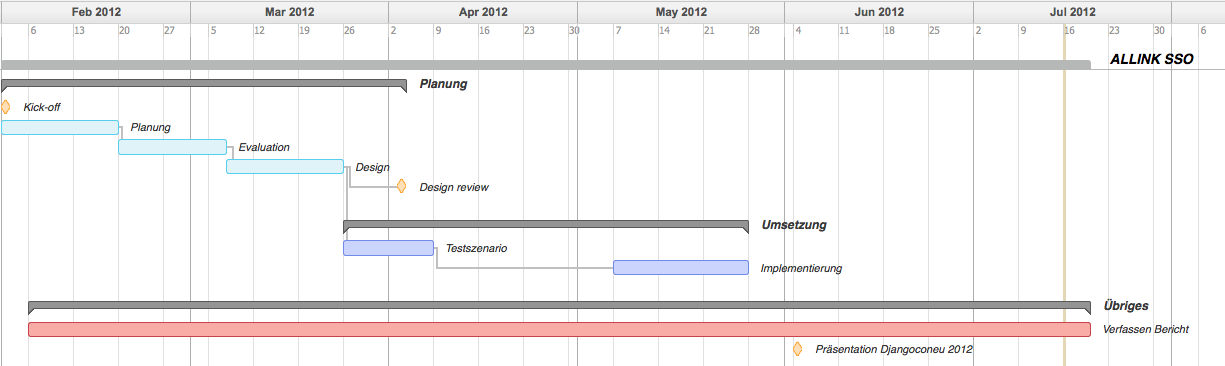
\includegraphics[width=21cm, angle=90]{include/zeitplan.png}
	\caption{Zeitplan}
	\label{fig:zeitplan}
\end{figure}
